
%
\documentclass[conference]{IEEEtran}



\usepackage{cite}

%
\ifCLASSINFOpdf
  \usepackage[pdftex]{graphicx}
  \usepackage{epstopdf}
  % declare the path(s) where your graphic files are
  % \graphicspath{{../pdf/}{../jpeg/}}
  % and their extensions so you won't have to specify these with
  % every instance of \includegraphics
  % \DeclareGraphicsExtensions{.pdf,.jpeg,.png}
\else
  % or other class option (dvipsone, dvipdf, if not using dvips). graphicx
  % will default to the driver specified in the system graphics.cfg if no
  % driver is specified.
  % \usepackage[dvips]{graphicx}
  % declare the path(s) where your graphic files are
  % \graphicspath{{../eps/}}
  % and their extensions so you won't have to specify these with
  % every instance of \includegraphics
  % \DeclareGraphicsExtensions{.eps}
\fi






% *** MATH PACKAGES ***
%
\usepackage[cmex10]{amsmath}

\usepackage{algorithm}
\usepackage{algorithmic}

%
\usepackage{array}



\hyphenation{op-tical net-works semi-conduc-tor}


\begin{document}
%
% paper title
% can use linebreaks \\ within to get better formatting as desired
% Do not put math or special symbols in the title.
\title{A Novel Link Scheduling Algorithm for Wireless Networks using Directional Antenna}


% author names and affiliations
% use a multiple column layout for up to three different
% affiliations

\author{\IEEEauthorblockN{Zhaoshu Tang, Ming Zhu, Lei Wang, Honglian Ma}
\IEEEauthorblockA{School of Software\\
Dalian University of Technology, China\\
tang.zhaoshu@mail.dlut.edu.cn, zhuming@dlut.edu.cn, lei.wang@dlut.edu.cn, mhl@dlut.edu.cn}
}
% conference papers do not typically use \thanks and this command
% is locked out in conference mode. If really needed, such as for
% the acknowledgment of grants, issue a \IEEEoverridecommandlockouts
% after \documentclass

% for over three affiliations, or if they all won't fit within the width
% of the page, use this alternative format:
%
%\author{\IEEEauthorblockN{Michael Shell\IEEEauthorrefmark{1},
%Homer Simpson\IEEEauthorrefmark{2},
%James Kirk\IEEEauthorrefmark{3},
%Montgomery Scott\IEEEauthorrefmark{3} and
%Eldon Tyrell\IEEEauthorrefmark{4}}
%\IEEEauthorblockA{\IEEEauthorrefmark{1}School of Electrical and Computer Engineering\\
%Georgia Institute of Technology,
%Atlanta, Georgia 30332--0250\\ Email: see http://www.michaelshell.org/contact.html}
%\IEEEauthorblockA{\IEEEauthorrefmark{2}Twentieth Century Fox, Springfield, USA\\
%Email: homer@thesimpsons.com}
%\IEEEauthorblockA{\IEEEauthorrefmark{3}Starfleet Academy, San Francisco, California 96678-2391\\
%Telephone: (800) 555--1212, Fax: (888) 555--1212}
%\IEEEauthorblockA{\IEEEauthorrefmark{4}Tyrell Inc., 123 Replicant Street, Los Angeles, California 90210--4321}}








% make the title area
\maketitle

% As a general rule, do not put math, special symbols or citations
% in the abstract
\begin{abstract}
For a given set of communication links whose senders transmit at a fixed power level, it is a hot problem to select a maximum set of links that can be transmitted simultaneously, which is known to be NP-hard. The existing algorithm only apply to the condition of omnidirectional transmission. This paper addresses the problem in a plane wireless network where the nodes use directional antennas under physical interference model. We develop a directional interference model applicable to such networks, and first propose the approximation algorithm to solve scheduling problem under this model. We proved the correctness of the algorithm by mathematical analysis. We have also proved the great advantages of using directional antenna by extensive simulations.
\end{abstract}

% no keywords

\begin{IEEEkeywords}
Link Scheduling, Directional Antennas, Physical Interference Model
\end{IEEEkeywords}

\IEEEpeerreviewmaketitle



\section{Introduction}
% no \IEEEPARstart

As we all know, link scheduling is the most fundamental and typical problem which can significantly influence network performance.Since Gupta and Kumar first studied on the methods to schedule links and enhance the capacity in Wireless Sensor Networks \cite{capacityGP}, lot of problems were proposed one after another. In the case of shared only one channel, a plurality of communication links transmission at the same time will lead to signal interference. In wireless network, link scheduling problem is to reduce the maximum interference when the links transmit simultaneously, and ensure the message can be successfully accepted by the receiving node. The main objective is to achieve efficient spatial reuse and increase network capacity, considering wireless interference among concurrently transmitting nodes.

The problem maximum link scheduling (MLS) is to seek a largest set of links from a given set A that can be scheduled simultaneously. Given a set of communication link requests $L = \{l_1, l_2, �� , l_n\}$, with $l_i$ denoting the $i$th link request. MLS intends to find a maximum subset of links $S \in L$ to be scheduled simultaneously, designated to one time slot, given a set of communication links with each having a unit traffic demand. This optimization problem is NP-hard proved by Goussevskaia \cite{geometric}. There are a lot of studies to this aspect, some better performance approximation scheduling algorithms have been proposed \cite{Capacity}.

By concentrating the energy in specific direction, opposed to omni-directional transmission, directional antennas can provide the benefits of increased range, reduced interference and increased spatial reuse of bandwidth. We can benefit from the advantages provided by directional antennas if the scheduling does not take into account the nature of the beam formation at each node.


In order to solve this problem, there are mainly two kinds of interference model are used. One of them is graph-based model \cite{moscibroda2006protocol}, including the protocol interference model, CTS/RTS model, K-hop interference model and so on. By localizing the interference of a transceiver on others, it is much easier to track and handle. Unfortunately, the graph-based interference model is too idealistic and simple so that there are many vital factors are ignored. Another kind of interference model is physical interference model \cite{maheshwari2008measurement}, which is also known as SINR (signal-to-interference-plus-noise-ratio) model. In physical interference model, the accumulative interference is considered and thus it is more close to the reality. However, when physical interference model is applied, it is much more complex to calculate and design algorithm. Most of the researches are based on graph-based models which is too optimistic. To make our research more accurate, we adopted physical interference model in this paper.

As time goes on, much more conditions that will influence link scheduling performance significantly have been taken into account in the research, like power control which is a vital element. Many kinds of power control for instance, linear transmission power control, uniform transmission power control and arbitrary transmission power control are considered \cite{xu2012mlls}. Another important issue is about distribution or centralization problem. Most studies focus on the centralized implementation, but some develop distributed even localized link scheduling algorithms with provable throughput performance \cite{zhou2014throughput}.

In this paper, we apply directional antennas to the research of MLS problem based on the physical interference model, which can significantly reduce ambient interference and ensure more nodes can be transmitted at the same time. Then we also take full-duplex transmission into consideration, in which every node is both sender and receiver. It is more complex but also more realistic.



%
%The problem \emph{One-slot Maximum Set of Links} (OSML) is to seek a largest set of solution links from a given set $A$ that can be transmitted simultaneously. This optimization problem is NP-hard proved by Gussevskaia \cite{1}. Plenty of research to this problem, some approximation scheduling algorithms was be proposed \cite{1,2}, which is performance good.
%
%
%Nowadays, various ways to solve the problem of OSML under physical interference model was present. The author of \cite{1} designed the first non-trivial approximation algorithm with approximation bound $O(\log {\frac{\max_{l \in A }d(l)}{\min_{l \in A} d(l)}}) $. Goussevskaia made huge efforts on developing a constant approximation bound in the literature\cite{2}, which proposed a $O(\log {n})$ approximation for the problem of maximizing the number of links scheduled in one time-slot. Then, Peng-Jun Wan $et$ $al$., \cite{3} given a further analysis to the OSML problem under physical interference model. Besides, they summarize the method to solve this kind of problem in\cite{7}. Recently, more influential elements has been take into account in the experiment, like power control \cite{9}, throughput capacity and communication latency \cite{14}. Pei, Guanhong\cite{5} developed the first rigorous distributed algorithm for link scheduling in the SINR model. It uses physical carrier sensing and the distributed decisions are made based on the Received Signal Strength Indication (RSSI).
%
%
%However, mostly research of link scheduling based on omnidirectional transmission. Ramamurthi\cite{4} proposed a generalized physical interference model apply to the directional antennas, both take into account the main lobes and the side lobe of antennas. But the problem they focus is different from our research. The benefits of directional antennas to improve network capacity has been deep analysed in \cite{10}. Although directional antennas have been studied for cellular networks and has been deployed for cell-sectoring, rarely used for OSML problem.
%
%In this paper, we design a directional interference model applicable to directional antennas. Then we propose an approximation algorithm OSML to solve link scheduling problem based on directional interference model. We giving the correctness analysis, performance analysis and provides a sound mathematical proof to some special case. Finally, we also present the performance of the algorithm by simulation, which compared with a omnidirectional algorithm.
%
The rest of the paper is organized as followed. We describe related work in Section \uppercase\expandafter{\romannumeral2}. Section \uppercase\expandafter{\romannumeral3} give our directional interference model. In section \uppercase\expandafter{\romannumeral4}, we present scheduling algorithm for the problem of MLS and Full-duplex MLS, also provide mathematical analysis for the algorithm. Section \uppercase\expandafter{\romannumeral5} show the simulation results to illustrate the performance of our scheduling algorithm, and section \uppercase\expandafter{\romannumeral6} concludes the paper.

\section{Related Work}

Since Gupta and Kumar first studied on the methods to schedule links and enhance the capacity in Wireless Sensor Networks, three sub-problems were proposed one after another: maximum link scheduling (MLS) problem \cite{geometric}, maximum weighted link scheduling (MWLS) problem \cite{wan2010shortest} and shortest link scheduling (SLS) problem \cite{Capacity}. In the process of studying the scheduling problem, some other factors are also need to take account of, such as the interference, power control, centralized or distributed scheduling, omnidirectional or directional antennas and so on.

Goussevskaia et al. \cite{geometric} give us a simple proof that link scheduling under the SINR model is NP-hard. He also proposed an $O(l_{max} / l_{min})$ factor approximation algorithm for MLS problem with a uniform power assignment, where lmax and lmin denote the length of the longest and the shortest link, respectively. The algorithm used greedy strategy to construct a scheduling in different classes partitioned by length. After a while, Goussevskaia \cite{Capacity} made huge efforts on developing a constant approximation bound in the literature and proposed a $O(\log {n})$ approximation for the problem of maximizing the number of links scheduled in one time-slot scheduling. Then a factor of $O(1)$ -approximation ratio algorithm was put forward by Halld��rsson and Mitra \cite{generalmetrics}. They extended the transmission power to oblivious power assignment (including uniform, mean, and linear power assignment). Furthermore, the algorithm is applicable for both unidirectional and bidirectional links. In this paper, we will analyze bidirectional communication because bidirectional communication is more consistent with WSNs. Fanghanel et al. introduced the bidirectional version of the scheduling problem and gave a first polynomial time approximation factor algorithm for SLS using the mean power assignment in general metrics \cite{fanghanel2009oblivious}. This result was improved to $O(n\log {n})$ in \cite{halldorsson2012wireless}.

The links scheduling algorithms under SINR model are more accurate than that under the graph-based models since the physical interference model can accurately describe the interference in wireless networks. Considering the interference model used in Goussevskaia et al. (2007, 2009)[1,3], it is an approximation of the SINR model, but the effect of noise is ignored in this paper. SINR is simplified to SIR problem after neglecting the ambient noise, in which the transmission scope of a link will become infinite. In this way, the possible number of link classes divided by length is infinite as well. Blough et al. \cite{blough2010approximation} proposed the first SLS algorithm under the exact SINR model. He defined a class of links named ��black-gray�� links, whose lengths are equal or near to the maximum transmission scope of the sender. In the extreme case, in which all the links to be scheduled are ��black-gray��, they obtained an upper bound on the length of SLS algorithm, which is $O(|C_0| + \Delta_{max})$, where $|C_0|$is the number of links in class $C_0$, and $\Delta_{max}$ is the maximal number of receivers in a cell of class $C_k$. In \cite{li2008maximal} and \cite{li2012maximal}, Li proposed a hypergraph model combining graph-based model and SINR models, and demonstrated that the hypergraph model contains the advantages of both graph-based model and the SINR model while avoiding their drawbacks. Namely, the hypergraph model can emulate cumulative interference constraints as hyperedge, where each hyperedge is a set of links that are not allowed to transmit simultaneously. Thus, this model can avoid the defects of graph-based models which overlook the cumulative interference.

The algorithms mentioned above adopt uniform power assignment. Many algorithms for link scheduling with non-uniform power assignment are also addressed by people. Kozal et al.\cite{kozat2006cross} proved the problem of power control and scheduling to be NP-complete by using a reduction from integer programming under the assumption that the values of gain matrix can be chose arbitrarily. In Kesselheim \cite{kesselheim2011constant}, Kesslheim studied the capacity maximization problem with power control in a wireless network. With the objective of maximizing the number of simultaneous links to communicate, he developed an algorithm which selected a subset of links and chosen a power level for each link. He also proved that the algorithm achieves $\Omega(n)$, $\log(n)$ approximation in a fading metric and a general metric space, where $n$ is the number of links.

All the works reviewed by now are centralized, and the studies don��t give us a strategy to develop a distributed version. Le et al. \cite{le2010longest} proposed a distributed
greedy maximal link scheduling algorithm under interference localization. A link l only performs scheduling coordination inside a circle area named interference neighborhood of the link. However, the trivial procedure for determining the interference neighborhood is centralized. Moreover, link l and other links need to calculate their cumulative interference in an iterated procedure, which is impractical in a large scale network. Pei and Vullikanti \cite{(2012) [26]} proposed a local distributed scheduling and power control algorithm under the SINR model, achieving an $O(\log^2{n})$ approximation factor in the throughput region. Note that the uniform power assignment for all links was adopted, and thus the links in the same link class were assigned the same power. However, they do not give reasons why the number of active nodes in the vicinity of any active node decreases by half after each phase with a high probability.

However, mostly studies of link scheduling based on omnidirectional transmission. Ramamurthi \cite{directional} proposed a generalized physical interference model applying to the directional antennas, both taking into account the main lobes and the side lobes of antennas. The benefit of directional antennas to improve network capacity has been deeply analyzed in \cite{10}. Although directional antennas has been studied for cellular networks and has been deployed for cell-sectoring, it is rarely used for OSML problem.


\section{The Directional Interference Model}

An essential issue to link scheduling problem in wireless networks is the interference model. Here is a list of some notation meaning. All the networking nodes $V$ lie in plane and transmit at a fixed power $P$. The Euclidean distance between any pair of nodes is denoted by $d_{uv}$. The antenna gain of the node $u$ is $G_u$. The path loss model is then determined by the path-loss exponent $\alpha$, which is a constant greater than $2$ but less than $6$ typically. Specifically, when a node $u$ transmit a signal at power $P$, the power of this signal is captured by another node $v$ is $P d^{-\alpha}_{uv} G_u G_v$. The signal quality perceived by receiver is measured by the SINR (signal to interference and noise ratio), which is the quotient between the power of the wanted signal and the total power of unwanted signals and the ambient noise (both internal and external).

Here is a brief introduce to independent set. It is a set of disjoint links that can be scheduled at a same time slot, formulated as follows. A set of links $S=\{ (u_1,v_1),(u_2,v_2),...,(u_k,v_k) \}$ are said to be independent if:

(1) all links in $S$ are disjoint;

(2) for each $1 \leq i \leq k$, the SINR of the link $u_i,v_i$ with respect to ${u_j:1 \leq j \leq k,j \neq i}$ is at least $\beta$.

\emph{1) physical interference model \cite{11}:} In this model, the transmission from sending node $s_v$ is successfully received by receiver $r_v$ if and only if
\begin{equation}
  \textrm{SINR}=\frac{P d^{-\alpha}_{vv}}{N+ \sum _{l_w \in S}P   d^{- \alpha}_{wv} } \geq \beta,
\end{equation}
where $\alpha >2$ is the path-loss exponent, $\beta >1$ is the minimum SINR required for successful reception and determined by the hardware conditions, $N$ is the ambient noise around receiving node (note that $\alpha,\beta,N$ are all constants). This models a situation where the SINR must be no less than certain threshold $\beta$, in order to correctly interpret the wanted signal. It is a very effective model for omnidirectional transmission, takes the total interference into account due to all transmissions.

In our search, each nodes sending by directional antenna but received by omni-directional antenna. The problem of OSML can be formulated as follows. Given a set of links $L=\{l_1,l_2,...l_n\}$, where each link $l_i$ represents a communication request from a sender node $s_i$ to a receiver $r_i$, and our object is to seek a maximum independent set in one time-slot, that means each links in the independent set can be scheduled simultaneously.

We assume the length of link $l_v$ is denoted by $d_{vv}$, and simplify directional antennas as only have one main beam, fixing the direction of the antenna. Which the interference range only in a particular angle generated by sending node.


\emph{2) direcional interference model \cite{11}:} The link $l_v=(s_v,r_v)$ successfully transmitted under the following conditions:\\
(1) In the absence of other links:
\begin{equation}
\textrm{SNR}=\frac{PG_{s_v} G_{r_v} d^{-\alpha}_{vv}}{N} \geq \beta.
\end{equation}
(2) Presence of interference from other links:
\begin{equation}
  \textrm{SINR}=\frac{PG_{s_v} G_{r_v} d^{-\alpha}_{vv}}{N+ \sum _{l_w \in S}P G_{s_w} G_{r_v} d^{- \alpha}_{wv} \varphi _{wv}} \geq \beta,
\end{equation}
where $P$ is transmission power of the transmit node, link $l_w \in S$ scheduled concurrently with $l_v$, $G_{s_v}$ and $G_{r_v}$ is the antenna gain of sending node and receiving node, it is a constant which deceive by hardware conditions.

\begin{figure}[!t]
\centering
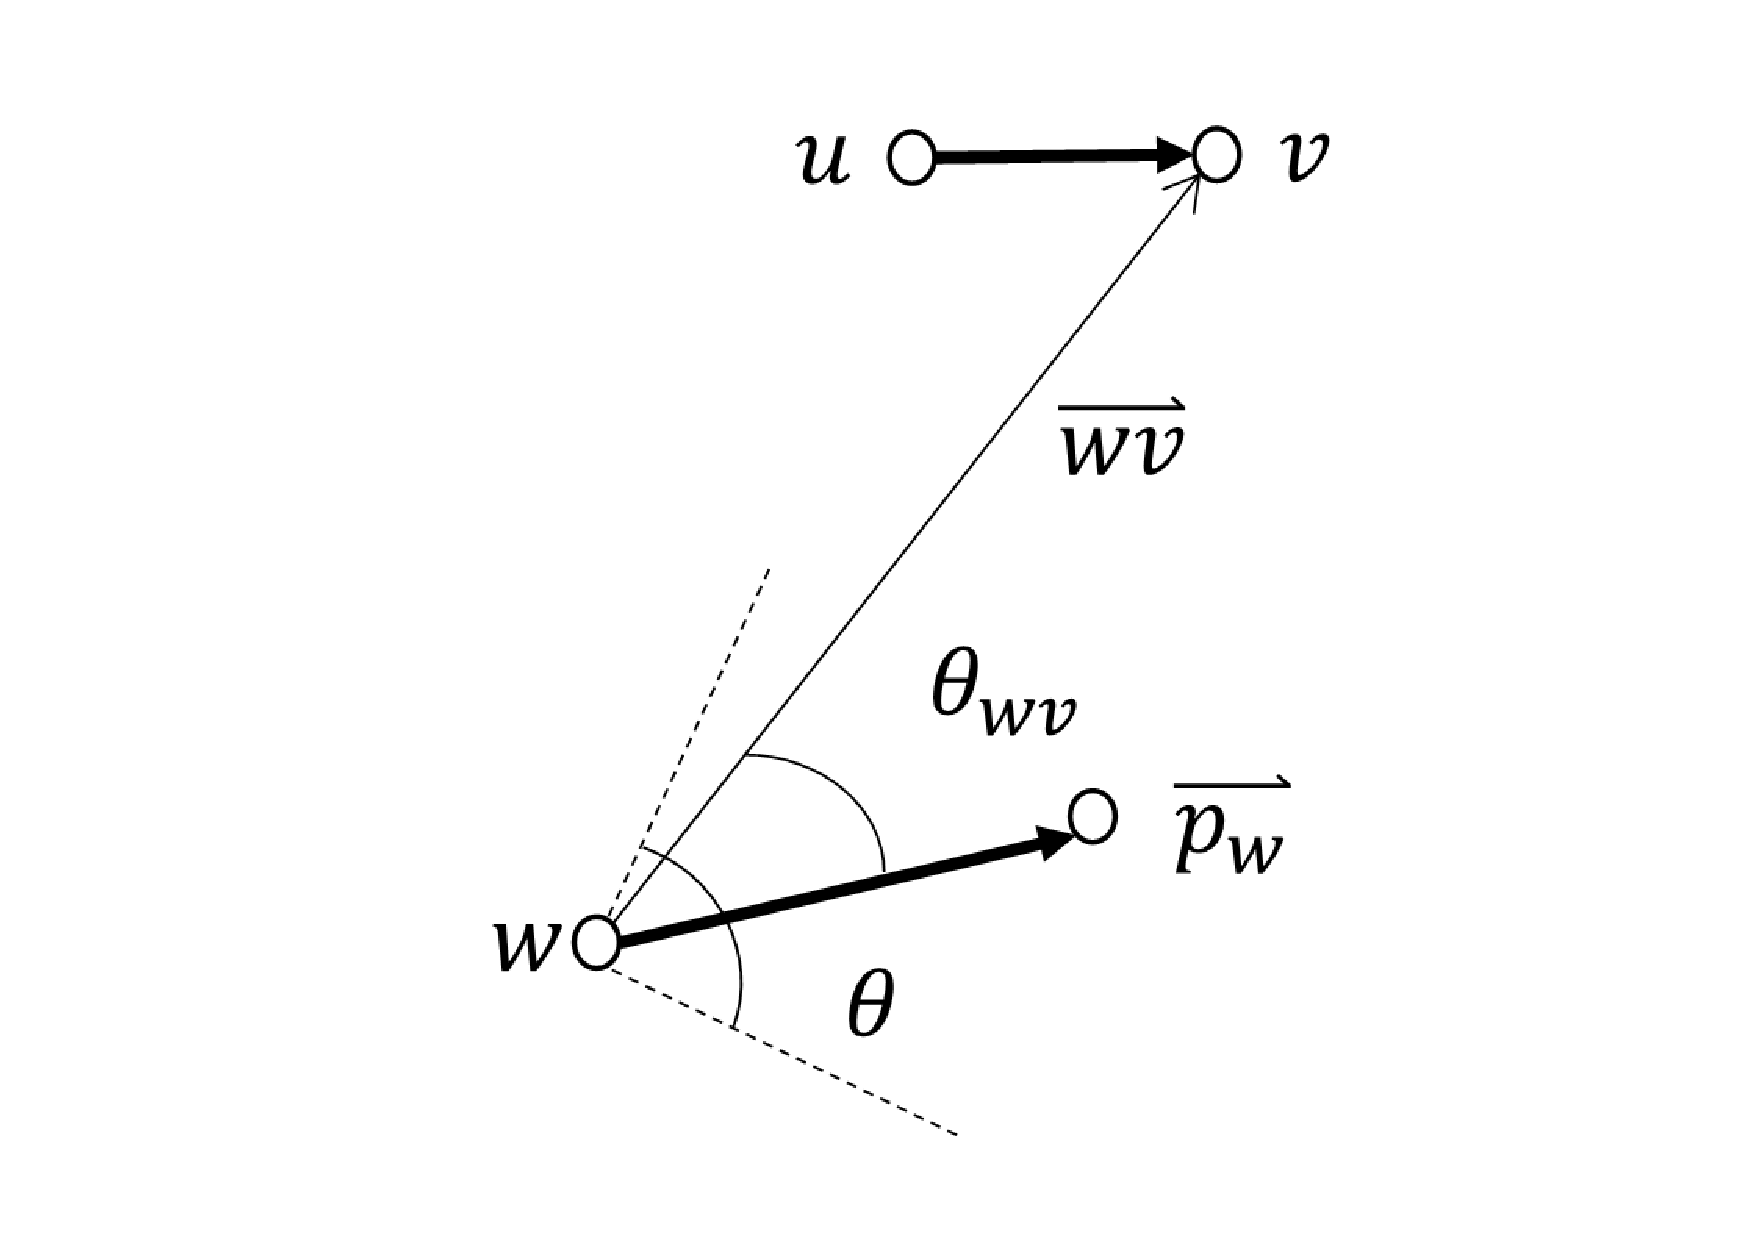
\includegraphics[width=3in]{image/direction.pdf}
% where an .eps filename suffix will be assumed under latex,
% and a .pdf suffix will be assumed for pdflatex; or what has been declared
\DeclareGraphicsExtensions.
\caption{Angle Judge.}
\label{Angle Judge}
\end{figure}

The model was proposed to narrow the interference angle by using directional antenna, so we need to determine whether exist interference between the links that transmission in the same time. Here we use $\varphi _{wv}$ to solve this problem, where vector $\vec {p_w}$ present the send direction of node $w$, the send angle of directional antennas is $\theta _w$. Definition as follows:
\[
\varphi =\left \{ \begin{split}
0 &, \theta_{wv}>\theta_w /2,\\
1 &, \theta_{wv}\leq \theta_w /2,
\end{split}
\right.
\]
where $\theta _{wv}$ is the angle between antenna direction $\vec {p_w}$ of sender node $w$ with the vector $\vec {wv}$ that the direction of sender node $w$ to receiver node $v$. We use this angle to judge whether the receiving node is in the send range of the sender node. As shown in Fig. \ref{Angle Judge}. We can use the following formulate to get the angle $\theta_{wv}$, and decide the interference between links.
\begin{equation*}
  \theta_{wv}=\arccos{(\frac{\vec{p_w} \vec{wv}}{|\vec{p_w}| |\vec{wv}|})}.
\end{equation*}

In this research, we assume that all nodes transmit with the same power level $P$. There are some definition, use $P_{vv}=PG_sG_r/d^{\alpha}_{vv}$ represent the signal receive power of $r_v$ send by $s_v$, and $I_{wv}=P G_{s_w} G_{r_v} \varphi_{wv}/d^{\alpha}_{wv}$ denote the signal interference received by node $r_v$ from a sender $s_v$ that transmit at the same time.


% You must have at least 2 lines in the paragraph with the drop letter
% (should never be an issue)

\section{The Scheduling Algorithm}

In order to solve the scheduling problem of MLS, we present the follow LSDA(Link Scheduling Algorithm based on Directional Antenna) algorithm. Start with some definitions, the \emph{relative interference} (RI) of a link $l_u$ on link $l_v$, namely $RI_u(v)=I_{uv}/P_{vv}$. The \emph{affectedness} (proposed in \cite{2}) of link $l_v$, caused by a set of links $S$, is the sum of the relative interferences of the links in $S$ on $l_v$, as well as the effect of noise, scale by $\beta$, or
\begin{equation}
\begin{split}
  A_S(l_v)&=\beta \bigg(\frac{N}{P_{vv}}+\sum _{l_u \in S}RI_u(v)\bigg)\\
  &=\beta \frac{\sum_{l_u \in S}I_{uv}+N}{P_{vv}}.
\end{split}
\end{equation}

The formula of \emph{affectedness} was got from $\textrm{SINR} \geq \beta$. Observe that the \emph{affectedness} of link $l_v$ satisfy $A_S(l_v)\leq 1$, equivalent to the $\textrm{SINR} \geq \beta$, means link $l_v$ can successful transmission.

\begin{algorithm}
\caption{LSDA Algorithm}
\label{alg1}
\begin{algorithmic}[1]
\REQUIRE Set of links in the increasing order of length $L={l_1,l_2,...,l_n};$ $S \leftarrow \emptyset,$ $I \leftarrow \emptyset,$ $L_1 \leftarrow \emptyset$.
\ENSURE OMSL schedule $S$.
\STATE Set c according to Eq. (\ref{value of c}).
\REPEAT
\STATE $l_v=(s_v,r_v) \leftarrow$ the first link in $L$.
\STATE $L \leftarrow L \backslash {l_v},$ $S \leftarrow S\cup {l_v}$.
\STATE $L_1 \leftarrow l_u \in L:$ $d(s_u,r_v) \leq c \cdot d_{vv},$ $\varphi_{uv}=1$.
\STATE $L \leftarrow L \backslash L_1$.

\REPEAT
\STATE $l_w \in L \leftarrow$ satisfy $\varphi_{wv}=1$.
\STATE $I \leftarrow I \cup {l_w}$.
\UNTIL{$L$ is traversal end.}

\REPEAT
\STATE $l_a=(s_a,r_a) \leftarrow$ the first link in $I$.
\STATE $I \leftarrow I \backslash l_a$.
\REPEAT
\STATE $I_a \leftarrow l_u \in I:$ $d_{ua}=d(s_u,s_a) \leq  d_{aa}/2$.
\STATE $I \leftarrow I \backslash I_a$.
\STATE $L_v \leftarrow I_a \cup L_2$.
\UNTIL{$I$ is traversal end.}
\UNTIL{$I=\emptyset$. }

\STATE $L \leftarrow L \backslash L_v$.
\STATE Set $I \leftarrow \emptyset$.
\STATE $L_2 \leftarrow l_u \in L:$ $A_S(l_u) \geq 2/3$.
\STATE $L \leftarrow L \backslash L_2$.
\UNTIL{$L=\emptyset$.}
\RETURN $S$.
\end{algorithmic}
\end{algorithm}

Our approximation algorithm for LSDA is outlined above. We can simplify the algorithm as a brute-force method. Let $L$ be the set of given communication links, we assume that each link $l_v\in L$ can success communication, added to the solution, its safety ($\textrm{SINR} \geq \beta$) is guaranteed in the step of select. Set $L$ is a sequence which sorted in the increasing order of length of links. Depend on the definition of SINR, we can get the feature that the shorter the length, the more stable of the link. $S$ stores the link in one of independent set, and $I$ is the set of links have interference with the select link $l_v$ in each iterative. In every iteration of the algorithm, there have three step to select the legal and remove illegal link. The first link $l_v$ in $L$ is moved from $L$ to $S$, and use this link as the begin of the first round of selection. The first step (line 6) we need discards all links $l \in I$ whose sender are close to the receiver of $l_v$, meaning $d(r_v,s_w) \leq c \cdot d_{vv}$ ($c$ is a constant bigger than 2, and explained in next part).
\begin{equation}\label{value of c}
c=\max{  \bigg( 2,(2 \cdot 3^3 \cdot \beta \cdot \frac{\alpha-1}{\alpha-2})^{\frac{1}{\alpha-2}}\bigg)}.
\end{equation}
Then make sure the distance between any two links from set $I$ is bigger than $d_{vv}$, remove the illegal links from $L$ (line 16). The last step (line 23), all links $l_u \in L$, whose \emph{affectedness} $A_s(l_u)$ rose to or above a threshold of $2/3$, are removed from $L$ (the number of $2/3$ will explain in next part). This iterative is repeated until all links in $L$ have been select or deleted. In the end, we will get the scheduling set $S$ from LSDA algorithm. Next we prove that the obtained schedule is both correct and competitive.



\subsection{Correctness of Link Scheduling Algorithm}
In this section we prove that the solution $S$ obtained in LSDA Algorithm is correct, all selected links can be scheduled concurrently without collisions, $\forall l_v \in S$, $A_S(l_v) \leq 1$.

There some definitions need to be used in the proof. For link $l_v \in S$, let $S^-_v$ be the set of links that length shorts than $l_v$, and  $S^+_v$ be the links longer than $l_v$, there have some interference between $l_v$ and any link $l_w$ from $S^-_v$ or $S^+_v$ ($\varphi_{wv}=1$).

We can get from third part in iteration of the algorithm (line 22), each link in the scheduling set $S$ satisfy that the \emph{affectedness}, $A_{S^-_v}(l_v) \leq 2/3$, means that for each links $l_v \in S$, when the link is add to the set $S$, the \emph{affectedness} of $l_v$ get by $S^-_v$ is less than $2/3$, since it has not been deleted by in the previous step. In order to ensure that each links in $S$ can be successful communication at the same time slot, the SINR of each link should be satisfy $\textrm{SINR} \geq \beta$. It show that we just need to ensure $\forall l_v \in S $, $ A_{S^+_v}(l_v) \leq 1/3$.

In order to give a clear analyse, here are some geometric definition now. We used $D_w$ present the discs of radius $d_{ww}/2$ around receiver node $s_w \in S^+_v$. From the first elimination criterion, we know the discs $D_w$ do not contain any sender $s_z \neq s_w$ and $s_z \in S^+_v$. Focus on the links set $I$ which have interference on link $l_v$. At the first, division the sender set in $I$ into concentric rings $Ring_k$ which have evenly spaced of $cd_{vv}$ around the receiver $r_v$. Each ring $Ring_k$ contains all senders $s_w \in S^+_v$, for which $k(cd_{vv}) \leq d_{wv} \leq (k+1)(c d_{vv})$. Because of $d_{wv} \geq c \cdot d_{vv}$, so that the first ring $Ring_0$ does not contain any sender from $S^+_v$. Consider all senders $s_w \in Ring_k$, for the concentric rings $Ring_k$, $k>0$. All discs $D_w$ of radius $d_{vv}/2$ around node $s_w$ which located in $Ring_k$ must be completely contained in an extended ring $EXRing_k$, and the area is calculated by the fellow formula:
\begin{equation*}
\begin{split}
A(EXRing_k)&=[(d_{vv}(k+1)c+ d_{vv}/2)^2\\
&   - (d_{vv}kc - d_{vv}/2)^2]\pi  \\
&=c(2k+1) (c+1) d^2_{vv}\pi.
\end{split}
\end{equation*}

Since that each around discs $D_w$ of area $A(D_w) \leq d^2_{vv}\pi/4$ around senders $s_w \in I$ do not intersect, and the minimum distance between $r_v$ and $s_w$ is $k \cdot c \cdot d_{vv}$, $s_w \in Ring_k$, $k>0$. The total interference coming from ring $Ring_k$, $k>1$ is bounded by
\begin{equation*}
\begin{split}
I_{Ring_k}(l_v)&\leq \sum_{s_w \in Ring_k} I_{s_w}(l_v)\\
&\leq \frac{A(EXRing_k)}{A(D_w)}\cdot \frac{PG_{s_w}G_{r_v}\varphi_{wv}}{(kcd_{vv})^{\alpha}}\\
&\leq \frac{4(2k+1)(c+1)c}{k^{\alpha}c^{\alpha}}
\cdot \frac{PG_{s_w}G_{r_v}\varphi_{wv}}{(d_{vv})^{\alpha}}\\
&\leq \frac{1}{k^{\alpha -1}} \cdot \frac{1}{c^{\alpha-2}}
\cdot \frac{PG_{s_w}G_{r_v} \varphi_{wv} }{d^{\alpha}_{vv}} \cdot  3^2 \cdot 2.
\end{split}
\end{equation*}
The value of $PG_{s_w}G_{r_v}\varphi_{wv}$ is fixed in above deduce. $A(EXRing_k)/A (D_w)$ represent the maximum number of links have interference to link $l_v$ in the ring $Ring_k$, and we choose $d(s_w,r_v) =k(cd_{vv})$ ensure the interference to $l_v$ is the maximum. The last inequality holds since $k \geq 1$ and $c \geq 2$, obtain $2k+1 \leq 3k$ and $c+1 \leq 3c/2$. Summing up the interferences over all rings yields
\begin{equation*}
\begin{split}
  I_{S^+_v}(l_v)& < \sum_{k=1,...n} I_{Ring_k}(l_v)\\
  &\leq \sum_{k-1,...n} \frac{1}{k^{\alpha -1}} \cdot \frac{1}{c^{\alpha-2}} \cdot \frac{PG_{s_w}G_{r_v}\varphi_{wv}}{d^{\alpha}{vv}} \cdot 2\cdot3^2  \\
  &<\frac{\alpha -1}{\alpha-2} \cdot \frac{1}{c^{\alpha-2}} \cdot \frac{PG_{s_w}G_{r_v} \varphi_{wv}}{d^{\alpha}_{vv}} \cdot 2 \cdot 3^2,
\end{split}
\end{equation*}
where the last inequality holds since $\alpha >2$. This results in affectedness
\begin{equation*}
\begin{split}
  A_{S^+_v}(l_v) & =\beta \cdot \frac{\sum_{l_u \in S^+_v}RI_u(v)+N}{P_{vv}}\\
 & =\beta \cdot \frac{I_{S^+_v}(l_v)+N}{P_{vv}}\\
 & <\frac{\alpha-1}{\alpha-2} \cdot \frac{2 \cdot 3^2}{c^{\alpha-2}} \cdot \frac{1}{P_{vv}} \cdot \frac{PG_{s_w}G_{r_v} \varphi_{wv}}{d^{\alpha}_{vv}}\\ &+\frac{N \cdot \beta}{P_{vv}}\\
  \end{split}
\end{equation*}

In order to simplify the analysis, assume that there have no ambient noise $N=0$, antennas gain and the sending power of each nodes were fixed value.
\begin{equation}\label{refer C}
\begin{split}
A_{S^+_v}(l_v)=\frac{\alpha-1}{\alpha-2} \cdot \frac{2 \cdot 3^2}{c^{\alpha-2}} \cdot \beta \leq 1/3 \Rightarrow \\
c=\max { \bigg( 2,(2 \cdot 3^3 \cdot \beta \cdot \frac{\alpha-1}{\alpha-2})^{\frac{1}{\alpha-2}}\bigg)}.
\end{split}
\end{equation}

We have shown that each $l_v \in S$, satisfy $A_S(l_v) = A_{S^-_v}(l_v) + A_{S^+_v}(l_v) \leq 2/3 +1/3=1$, which means that $\textrm{SINR} \geq \beta$ for each link in scheduling set $S$. From above mathematical analysis, the value of $c$ was depend on design of third elimination part in algorithm. The judgement of $A_{S^-_v}(l_v) \leq 2/3$ just personal sense, and we proved the correctly.

\subsection{Algorithm Performance Analysis}
To analyze the performance of algorithm, we compared the solution $ALG$ of LSDA algorithm to an optimal solution, say $OPT$. Considering the complexity of directional transmission, we set some special case, and analyse the performance under those case. At first, give some lemma that satisfy the condition of omnidirectional antennas $\theta = 360^{\circ}$.

\emph{lemma 1}: Let $X$ be a feasible solution and let $l_v$ be a link in $X$. The number of sender nodes in $X$ within distance $k \cdot d_{vv}$, $k \geq 1$ of the receiver $r_v$ is at most $k^\alpha$.

\emph{Proof}: The relative interference of each sender $l_u \in X \backslash {l_v}$, where $d_{uv} \leq k \cdot d_{vv}$

\begin{equation*}
  RI_u(v)=\frac{I_{uv}}{P_{vv}}=\frac{P/d^\alpha_{uv}}{P/d^\alpha_{vv}}=(\frac{d_{vv}}{d_{uv}})^\alpha \geq \frac{1}{k^\alpha},
\end{equation*}
which means the maximum number is $k^{\alpha}$, otherwise the $\sum_{l_u \in X} RI_u(v) > 1$. Thus the lemma was been proved.

Then, we set other spacial case that communication angle is $\theta = 180^{\circ}$ of each nodes, and have the same orientation angle. Along with the direction of the orientation angle, the length of links getting shorter and shorter. In this case, the shortest link have no influence to the transmission of other links, which means the last elimination step (line 23) of algorithm have no effect, but get the interference from the larger length of links. $ALG_{180}$ represent the solution of LSDA algorithm, and $OPT_{180}$ is the optimal solution in the same condition.

\emph{lemma 2}: In $k$th iteration of the algorithm, we got one link to the solution $ALG_{180}$ and $|OPT_k| \leq (c+(k-1)/2)^{\alpha}$, $OPT_k$ was the optimal solution in $k$th iteration.


\emph{Proof}: Due to the special condition, we just need analyse the first and second elimination part in the algorithm. Consider the set $X_v \subseteq OPT_{180}$ eliminated in the first part of algorithm (line 6), in the iteration when link $l_v \in ALG_{180}$ was added to the scheduling solution. Each link $l_w \in X_v$ is of length at least $d_{vv}$, and the distance of its sender at most $c \cdot d_{vv}$ from receiver $r_v$. By \emph{Lemma 2}, there can be at most $c^{\alpha}$ in the set $X_v$.

For the second part of the proof, which equivalent to a pretreatment for the next iteration of the algorithm. Consider the set $L_v \subseteq L$ that the length of each links bigger than the link $l_v \in ALG_{180}$. In this part of eliminated, ensure the distance of each sender of links at least $d_{vv}/2$. We used the $Y_k$ represent the links which exist in second part of elimination at $k$th iteration, and the $d_k$ is the distance of the $k$th iteration when link $l_k \in ALG_{180}$ added to the scheduling solution, $d_k= d(l_k)/2$.

Combine the result of the last iteration. In the $k$th iteration, it is possible that the links in the discs around $l_w \in Y_k$ was been delete with the radius at most $R_k$. In the first iteration, the radius $R_1 = d_1= d(l_1)/2 \leq d_k$. If $k=2$, $R_2= R_1+ d_2 \leq 2 d_k$. From the induction result, in the $k$th iteration, which $l_v$ added to the solution. At worst, maybe delete all the links in the discs of radius $R_k=R_{k-1} + d_{vv}/2 \leq k \cdot d_{vv}/2$ around each sender $s_w \in Y_k$.

In general, during the process of $k$th iteration, $l_v \in ALG_{180}$ was the legal link. Combine the first part and second part of elimination. Each link $l_w \in X_v$ is of length at least $d_{vv}$ and has its sender of distance at most $c \cdot d_{vv} + (k-1) \cdot d_{vv}/2$ from receiver $r_v$. Therefore, can be at most $(c+(k-1)/2)^{\alpha}$ senders in $X_v$.

Due to the complexity of the directional antennas, we can not offered generally demonstration for the algorithm. But the number of non-intersect links is the least number of scheduling links. In other words, all of the non-intersect links can be scheduling at the same time.


\subsection{Full-duplex Algorithm}

Nowadays most of the researches about MLS problem are under unidirectional communication model which is more idealized and easy to tackle. However when it comes to the full-duplex transmissions, i.e. each node is able to send and receive signal at the same time, things are more complex. Because all links can behave as the sender and the receiver, the former definition of $\varphi$ is inappropriate. So we need to redefine some symbols and put forward a new algorithm which is suitable for the full-duplex transmissions situation.

First of all, we redefine the means of $\varphi$ as:
\[
\varphi =\left \{ \begin{split}
\infty &, \theta_{wv}>\theta_w / 2,\\
1 &, \theta_{wv} \leq \theta_w / 2,
\end{split}
\right.
\]
Then define the distance between the sending node $s_v$ and receiving node $r_u$ as $D_{s_v,r_u} = d (s_v, r_v) \cdot \varphi$, and we redefine the the distance between two links $l_v$ and $l_u$ as $D(l_v, l_u) = min\{D_{s_v, r_u}, D_{s_v, s_u}, D_{r_v, s_u}, D_{r_v, r_u}\}$. The $affectedness$ is calculated by the follow formula:
\begin{equation}
\begin{split}
  A_S(l_v)&=\beta \bigg(\frac{N}{P_{vv}}+\sum _{l_u \in S}RI_u(v)\bigg)\\
  &=\beta \frac{\sum_{l_u \in S}I_{uv}+N}{P_{vv}}\\
    &= \beta \frac{\sum_{l_u \in S} P G_{s_u} G_{r_v} D^{-1}_{l_u, l_v} + N}{P_{vv}}.
\end{split}
\end{equation}

Before algorithm description, we consider the condition of full-duplex transmissions. If only two links $l_v$ and $l_v$ transmit concurrently, the sufficient condition of link $l_u$ communicating successfully is that $SINR_{min}(l_v) \geq \beta$. Then we give the definition of "border distance", which is the minimum distance of concurrently transmitting links.

\emph{Definition:} border distance($BD$): a radius depend on the distance of link $l_v$, which is a circle does not include any others.
\begin{equation}
BD(l_v) = ( 2^4 \cdot \pi \cdot \beta \cdot \frac{\alpha - 1}{\alpha - 2} )^{\frac{1}{\alpha}}
\end{equation}
By the definition of "border distance", in order to ensure links $l_v$ and $l_u$ can transmit at the same time, the distance between $l_v$ and $l_u$ should satisfy: $D(l_v, l_u) \geq BD(l_v)$.

Next, we will present the algorithm of FLSDA(Full-duplex Link Scheduling Algorithm based on Directional Antenna), which solved the extend problem of MLS. The FLSDA works as follows:

\emph{1)} First, the input is a set of candidate links $L = \{l_1, l_2, ... ,l_n \}$, which are ranked from shorted to the longest by the distance of link. We choose the first one $l_v$ in the candidate set delete from $L$, and put it into the output set $S$ as the first solution.

\emph{2)} Then, in order to make sure $SINR(l_v) \geq \beta$. The selection mechanism delete the link $l_u$ whose distance to $l_v$ is shorter than $BD(l_v)$ by border distance, $D(l_u, l_v) \leq BD(l_v)$.

\emph{3)} Pick up the links $l_u \in L$ which get interference by $l_v$ as links set $I$. We judge whether link $l_v$ influence link $l_u$ by formula: $D(l_v, l_u) < \infty$.

\emph{4)} Choose the shortest link $l_u \in I$ and delete the links whose distance to $l_u$ is shorter than $BD(l_v)$ from link set $L$ and $I$. Repeat this remove process until the distance between every two links in $I$ is larger than $BD(l_v)$.

\emph{5)} Next, we decide the inference to links $l_u \in L$ by the current solution. Delete all the links $l_u$ in $L$ which satisfy $A_S(l_u) \geq 2/3$.

\emph{6)} Repeat all above step until the set $L$ is empty, and output the solution which is a set can transmit at the same time.

The process of full-duplex link scheduling algorithm is similar to LSDA. So the correctness has been proved in before. Next section we show the performance of LSDA and FLSDA.

\section{Evaluations}
In this section, we evaluate the performance of our link scheduling algorithms through simulation analysis, and analyse the influence by the element of links number, directional angle, antennas gains and so on.  We also make compared with One-slot scheduling algorithm (OSSA proposed in \cite{Capacity}) to show the performance.

To simplify the analysis of experiment result. We list the following conditions:
(1) All of the links random distributed on a plane field of size $1000*1000$ units (see Fig. \ref{Simulated Topologies}).
(2) All of the links transmit in the same power.
(3) In the experimental, we ignore the influence by ambient noise $N=0$.

\begin{figure}[t]
\centering
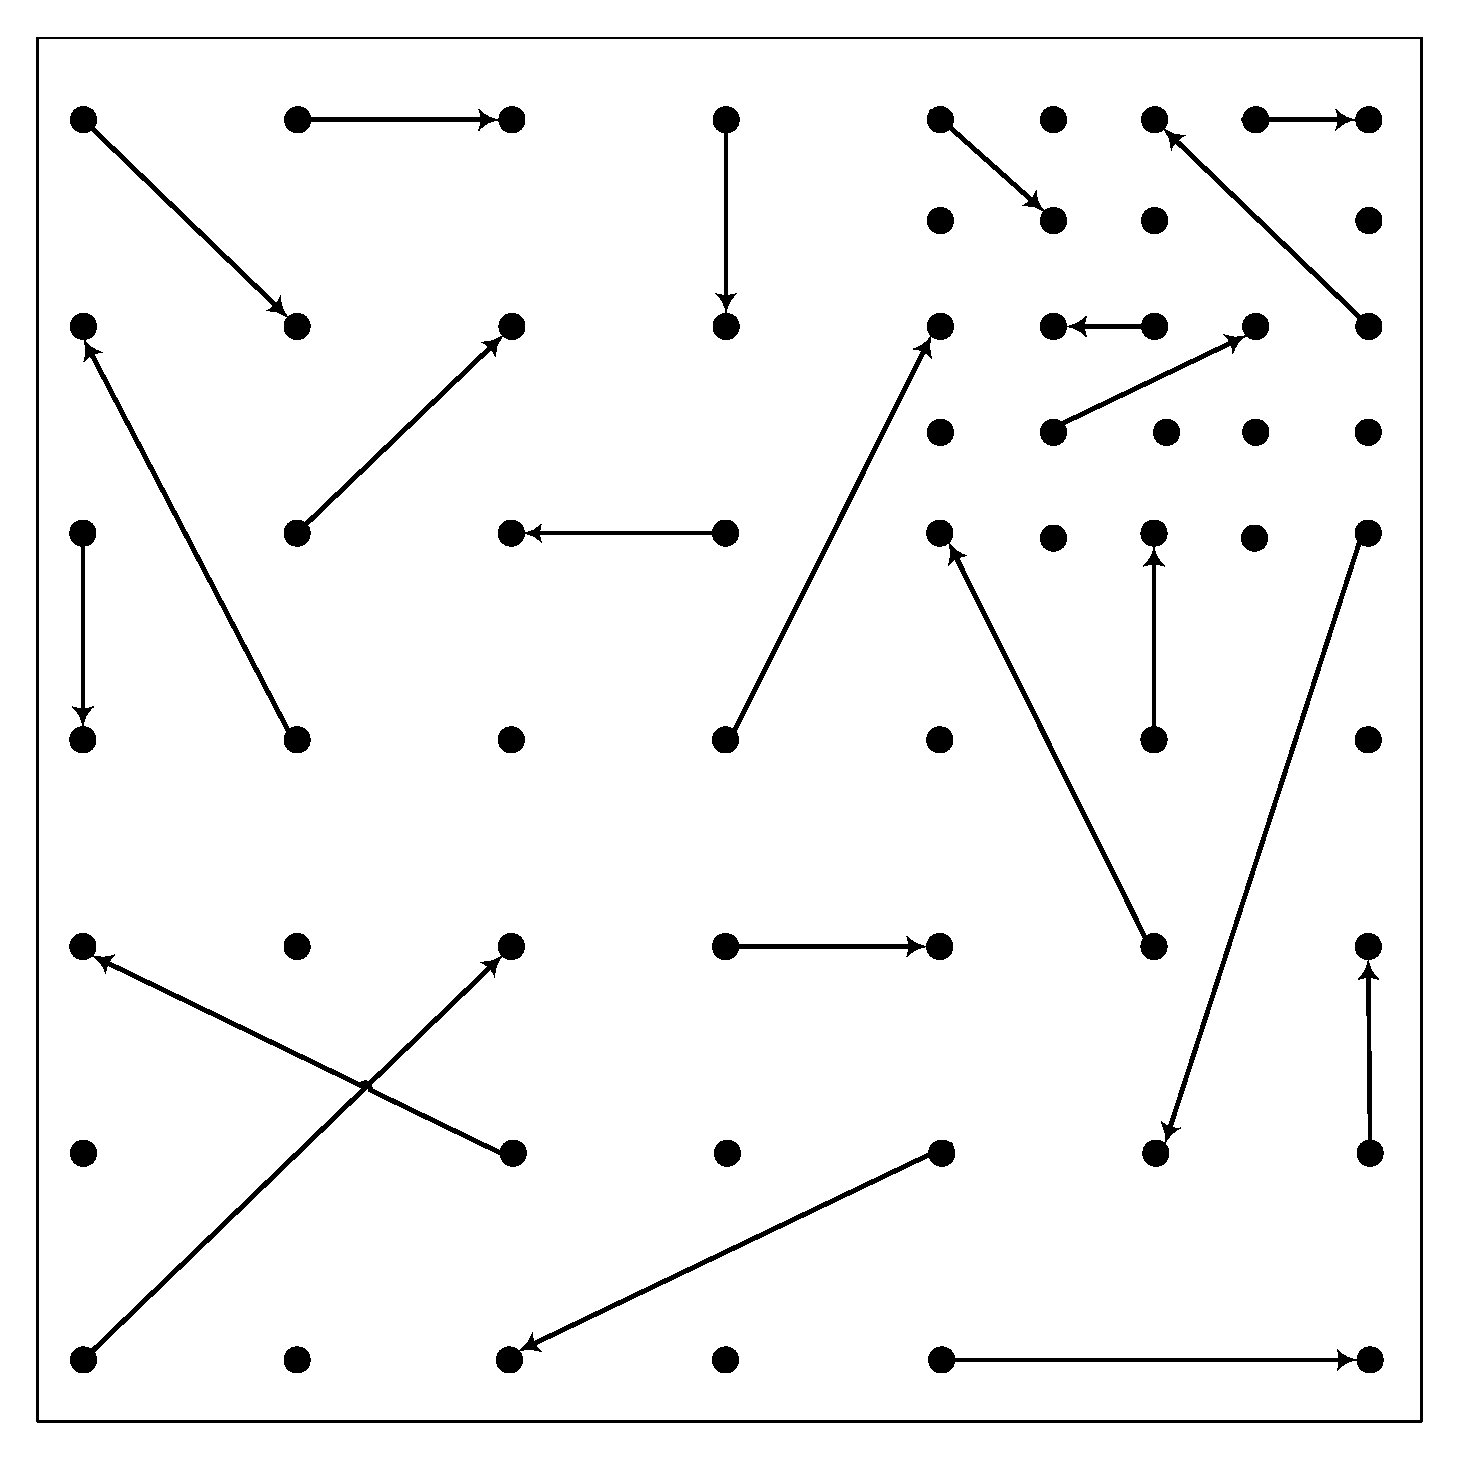
\includegraphics[width=2in]{image/topology.pdf}
% where an .eps filename suffix will be assumed under latex,
% and a .pdf suffix will be assumed for pdflatex; or what has been declared
\DeclareGraphicsExtensions.
\caption{Simulated Topologies.}
\label{Simulated Topologies}
\end{figure}


\begin{table}[h]
\centering
\caption{Default configuration parameter}
\label{parameter values}
  \begin{tabular}{|c|c|}
  \hline
  Parameter      &   Description  \\
  \hline
  Field         &   $1000 \time 1000$ units        \\
  Antenna Gain $G$       &   20dBi    \\
  Directional Angle $\theta$        &   $120^{\circ}$   \\
  Minimum SINR Required $\beta$        &   1.2    \\
  Path-loss Exponent $\alpha$        &   3    \\
  Power $P$         &   10w   \\

  \hline
  \end{tabular}

\end{table}


In our link scheduling algorithm, The size of the independent set present the performance of the algorithm. In our experiment, we using the size of output set as the performance standard, and the parameter values used in experiment is present as following (as shown in Table \ref{parameter values}).


\subsection{Experimental Results and Analysis}


\begin{figure}[htpb]
\centering
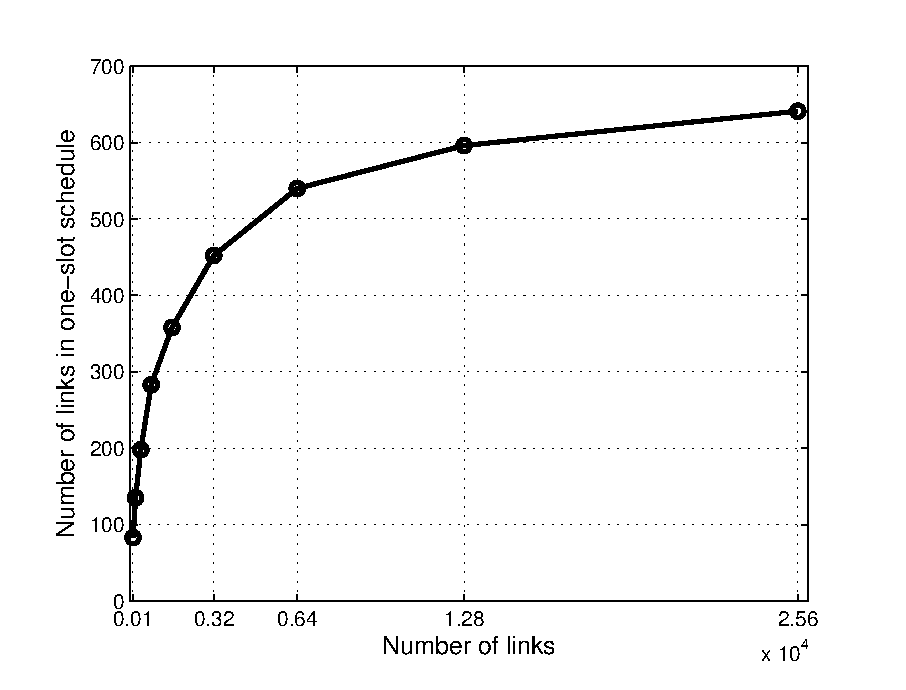
\includegraphics[width=2.5in]{image/1.eps}
% where an .eps filename suffix will be assumed under latex,
% and a .pdf suffix will be assumed for pdflatex; or what has been declared
\DeclareGraphicsExtensions.
\caption{LSDA Scheduling Algorithm. Nodes random distribution, $\theta = 120^{\circ}$, the number of links in one-slot schedule show the perform of the algorithm.}
\label{OSML Scheduling Algorithm.}
\end{figure}

In this subsection, we demonstrate that our algorithms LSDA and FLSDA via simulation study.

Assume that all nodes are deployed in a large network region. The length of links $l$ varies from 10 to 20 unit. Some important parameters are listed before. In our design, we fixed those parameters and increase the number of candidate links set to illustrate the performance of our algorithm. The results are shown in Fig. \ref{OSML Scheduling Algorithm.}, we analyse the influence by the size of the input set of links, and increase from $100 \times 2^0$ to $100\times 2^8$, $n \in \{100,200,400,800,1600,3200,6400,12800,25600\}$. In this experiment, we randomly create an input candidate links set which the size is $n$, and using the size of output set to evaluate the performance of LSDA. The simulation present that the size of the maximum independent set grows along with the increase of the number of the request link, but due to the limitations of the space, growth rate becomes slower and tends to balance.

We have a general impression to the performance of LSDA algorithm from above result. Then Now we give some results from other aspect to the algorithm. First, the influence of directional angle, the range of the angle satisfied $\theta \in \{30^{\circ},60^{\circ},90^{\circ},...,360^{\circ}\}$, and we make a comparison experiment $n=100$ and $n=3200$. In Fig. \ref{Influence of Directional Angle}. We known that the angle make a great influence to the performance of the LSDA scheduling algorithm, when other parameters were fixed. The smaller the angle, the better performance of the algorithm. In the case of maximum angle $\theta = 360^{\circ}$, the algorithm has a worst performance.

\begin{figure}[htpb]
\centering
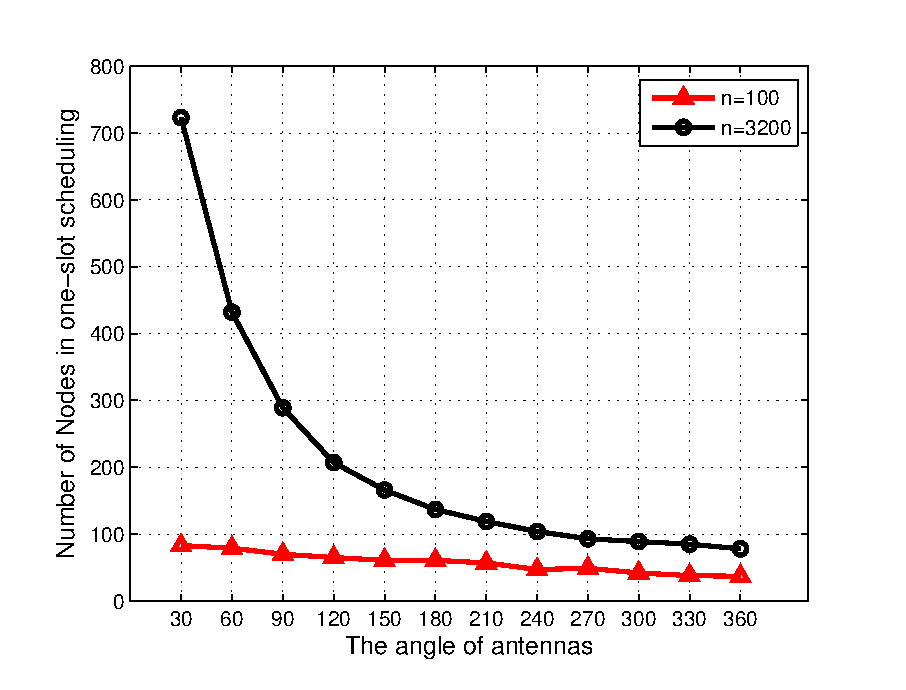
\includegraphics[width=2.5in]{image/3.eps}
% where an .eps filename suffix will be assumed under latex,
% and a .pdf suffix will be assumed for pdflatex; or what has been declared
\DeclareGraphicsExtensions.
\caption{Influence of Directional Angle. Change the angle of the directional antennas, compared the performance in high density with low density.}
\label{Influence of Directional Angle}
\end{figure}

\begin{figure}[!t]
\centering
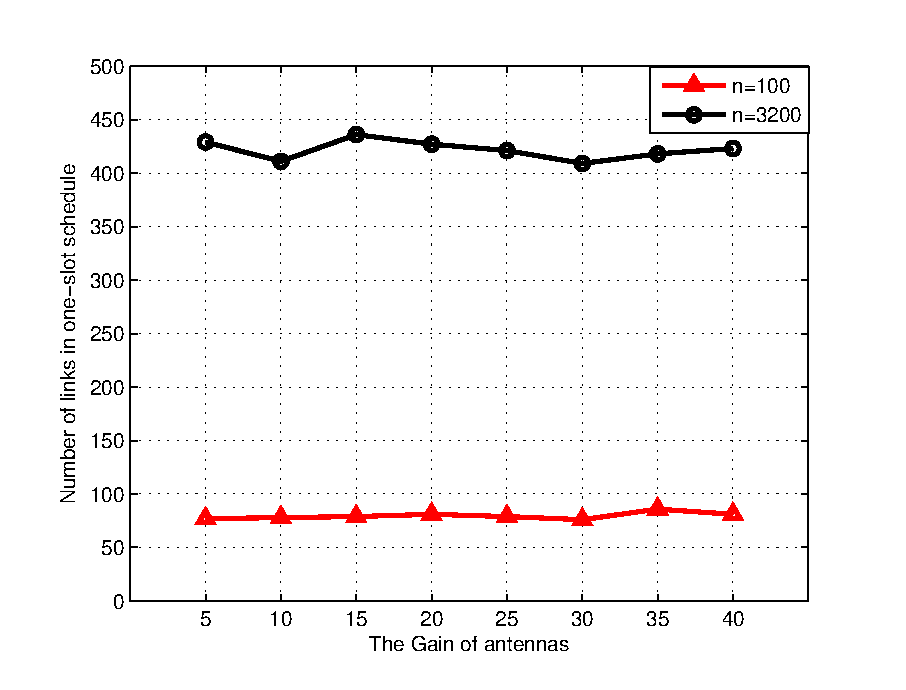
\includegraphics[width=2.5in]{image/4.eps}
% where an .eps filename suffix will be assumed under latex,
% and a .pdf suffix will be assumed for pdflatex; or what has been declared
\DeclareGraphicsExtensions.
\caption{Influence of Antenna Gain. Change the gain of the directional antennas, compared the performance in high density with low density.}
\label{Influence of Antenna Gain}
\end{figure}

Figure \ref{Influence of Antenna Gain} show the results of the influence to the algorithm by the antenna gain. We set up a fixed directional angle $\theta=60^{\circ}$, antenna gain $G \in \{5,10,15,20,25,30,35,40\}$, adopt double groups $n=100$, $n=3200$. According to the formula of SINR, we known that the changes of the antennas gain have a small effect to the result of algorithm. The simulation results shown that even if there have some fluctuation, the antennas gain have limited impact to the algorithm.

The above results were just get by separate analyzed of the OSML algorithm. Now we do some comparison between OSML algorithm and the one-slot scheduling algorithm. Parameter settings: $Gain=20$, $\theta =60^{\circ}$, and the number of links $n \in \{100,200,400,800,1600,3200,6400,12800,25600\}$. Shown in Fig. \ref{Comparison between OSML and One-slot Algorithm 1}, in random network topology, the performance of the OSML algorithm is batter than the one-slot algorithm. This is advantage of directional antennas, reduce the interference range by every nodes. In a fixed range of scene, more link can be allow for transmit together. In Fig. \ref{Comparison between OSML and One-slot Algorithm 2}, we change the angle of the antenna $\theta=360^{\circ}$, two curves of the algorithm are very similar in the condition of lower density, but slightly worse than one-slot algorithm in high density network. This performance is the comparison of the algorithm. OSML was designed to adapt the situation of direction. So the OSML has limited performance than other omnidirectional algorithm.

\begin{figure}[!t]
\centering
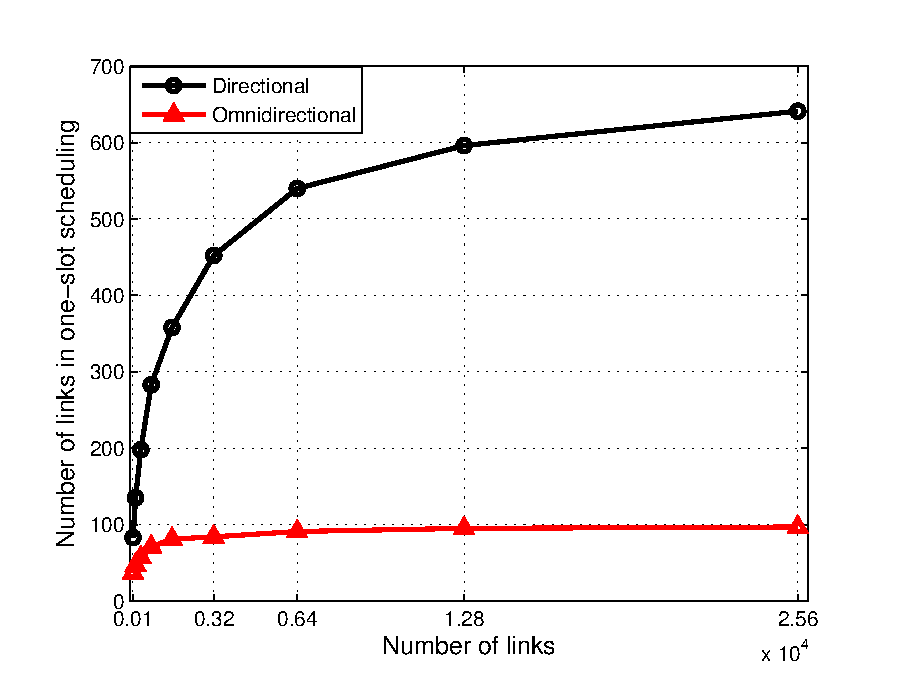
\includegraphics[width=2.5in]{image/5.eps}
% where an .eps filename suffix will be assumed under latex,
% and a .pdf suffix will be assumed for pdflatex; or what has been declared
\DeclareGraphicsExtensions.
\caption{Comparison between OSML and One-slot Algorithm. Use the same simulation data which generated at randomly by computer, but add the parameter of directional angle $\theta=60^{\circ}$ or $\theta=120^{\circ}$ when use to running OSML algorithm.}
\label{Comparison between OSML and One-slot Algorithm 1}
\end{figure}


To sum up, in random distribution wireless network, it has get an obvious effect to reduce the interference when multiple links transmission simultaneously by using directional antennas. The LSDA scheduling algorithm have better performance than this omnidirectional algorithm, and we also obtain that the antenna gain have a limited effect to the algorithm, but seriously influence by directional angle.

Now we take full-duplex transmission into consideration, the default configuration parameter were list in Table \ref{parameter values}. 

\begin{figure}[!t]
\centering
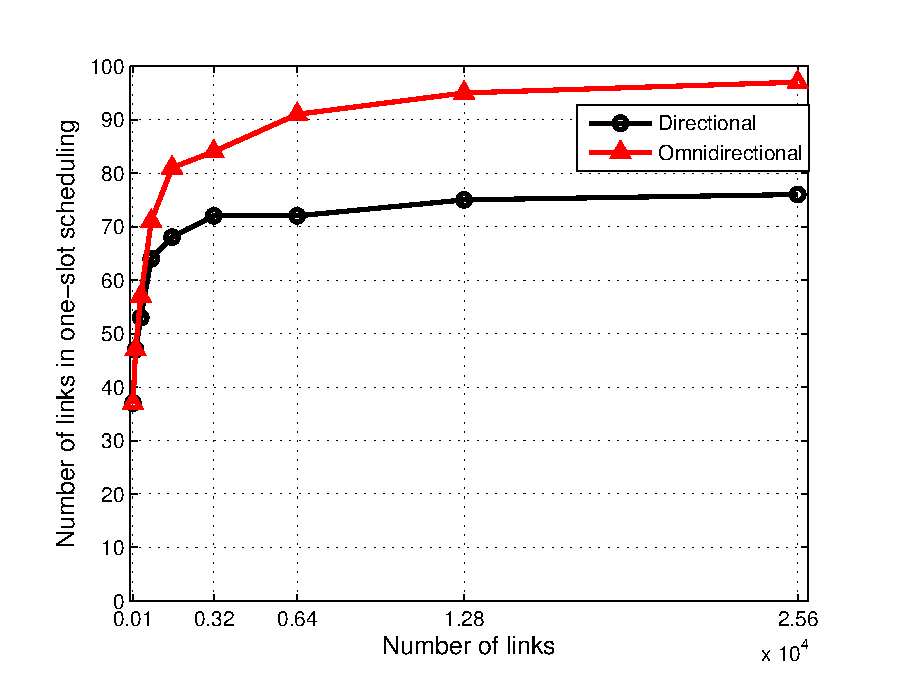
\includegraphics[width=2.5in]{image/6.eps}
% where an .eps filename suffix will be assumed under latex,
% and a .pdf suffix will be assumed for pdflatex; or what has been declared
\DeclareGraphicsExtensions.
\caption{Comparison between OSML and One-slot Algorithm. Set the directional angle $\theta=360^{\circ}$, which means use same random data running in different algorithm, compared the performance of two algorithm.}
\label{Comparison between OSML and One-slot Algorithm 2}
\end{figure}



\begin{figure}[htpb]
\centering
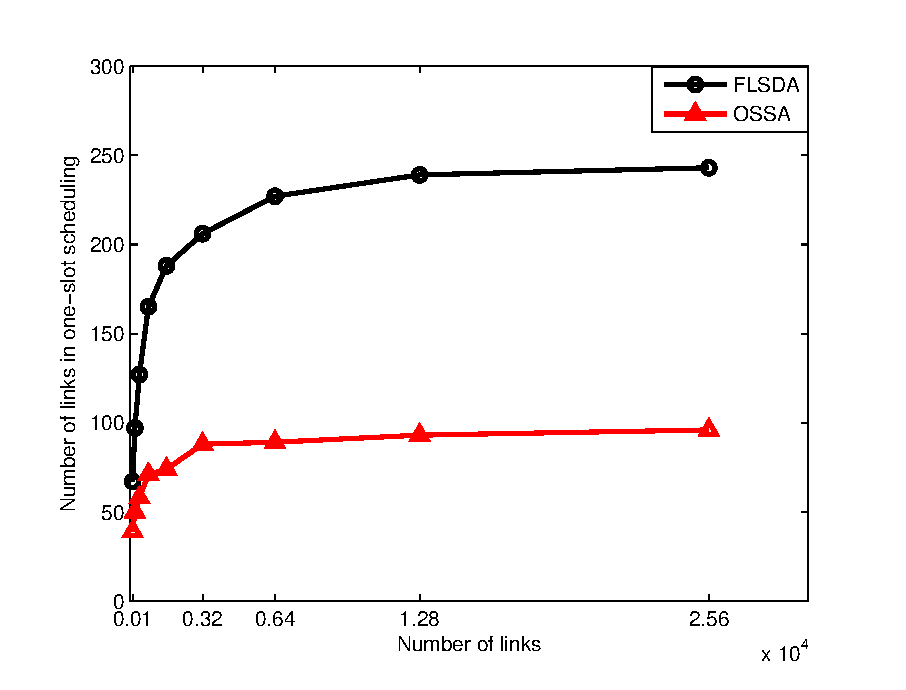
\includegraphics[width=2.5in]{image/bidirectional.eps}
% where an .eps filename suffix will be assumed under latex,
% and a .pdf suffix will be assumed for pdflatex; or what has been declared
\DeclareGraphicsExtensions.
\caption{Comparison between FLSA and OOSA.
Set the directional angle $\theta = 120^{\cdot}$, antenna gain G=20 and power=10 ,
which means use same random data running in different algorithm,
compared the performance of two algorithm.}
\label{Simulated Topologies}
\end{figure}

When take full-duplex into consideration, we have new results shown in Fig.8 and Fig.9. In Fig.8, we compared the bidrectional algorithm with OSSA while set number of links n �� {100, 200, 400, 800, 1600, 3200, 6400, 12800, 25600}, angle �� = 120?, antenna gain G=20 and power=10. From Fig.8 it��s obvious that two curves of the algorithm perform very close to each other when the density of the links is low. However the bidrectional algorithm behaves significantly much better than OSSA as the number of links increases and both of them tend to a fixed number and keep steady. In Fig.9 the directional angle �� = 120? and the link numbers=400, we can see that the influence of the change of path loss on the two algorithms is similar. Both of the results of two alogorithm keep increasing with the increase of the path loss exponent but the bidrectional alogorithm also performs better than OSSA.

% An example of a floating figure using the graphicx package.
% Note that \label must occur AFTER (or within) \caption.
% For figures, \caption should occur after the \includegraphics.
% Note that IEEEtran v1.7 and later has special internal code that
% is designed to preserve the operation of \label within \caption
% even when the captionsoff option is in effect. However, because
% of issues like this, it may be the safest practice to put all your
% \label just after \caption rather than within \caption{}.
%
% Reminder: the "draftcls" or "draftclsnofoot", not "draft", class
% option should be used if it is desired that the figures are to be
% displayed while in draft mode.
%
%\begin{figure}[!t]
%\centering
%\includegraphics[width=2.5in]{myfigure}
% where an .eps filename suffix will be assumed under latex,
% and a .pdf suffix will be assumed for pdflatex; or what has been declared
% via \DeclareGraphicsExtensions.
%\caption{Simulation Results.}
%\label{fig_sim}
%\end{figure}

% Note that IEEE typically puts floats only at the top, even when this
% results in a large percentage of a column being occupied by floats.


% An example of a double column floating figure using two subfigures.
% (The subfig.sty package must be loaded for this to work.)
% The subfigure \label commands are set within each subfloat command,
% and the \label for the overall figure must come after \caption.
% \hfil is used as a separator to get equal spacing.
% Watch out that the combined width of all the subfigures on a
% line do not exceed the text width or a line break will occur.
%
%\begin{figure*}[!t]
%\centering
%\subfloat[Case I]{\includegraphics[width=2.5in]{box}%
%\label{fig_first_case}}
%\hfil
%\subfloat[Case II]{\includegraphics[width=2.5in]{box}%
%\label{fig_second_case}}
%\caption{Simulation results.}
%\label{fig_sim}
%\end{figure*}
%
% Note that often IEEE papers with subfigures do not employ subfigure
% captions (using the optional argument to \subfloat[]), but instead will
% reference/describe all of them (a), (b), etc., within the main caption.


% An example of a floating table. Note that, for IEEE style tables, the
% \caption command should come BEFORE the table. Table text will default to
% \footnotesize as IEEE normally uses this smaller font for tables.
% The \label must come after \caption as always.
%
%\begin{table}[!t]
%% increase table row spacing, adjust to taste
%\renewcommand{\arraystretch}{1.3}
% if using array.sty, it might be a good idea to tweak the value of
% \extrarowheight as needed to properly center the text within the cells
%\caption{An Example of a Table}
%\label{table_example}
%\centering
%% Some packages, such as MDW tools, offer better commands for making tables
%% than the plain LaTeX2e tabular which is used here.
%\begin{tabular}{|c||c|}
%\hline
%One & Two\\
%\hline
%Three & Four\\
%\hline
%\end{tabular}
%\end{table}


% Note that IEEE does not put floats in the very first column - or typically
% anywhere on the first page for that matter. Also, in-text middle ("here")
% positioning is not used. Most IEEE journals/conferences use top floats
% exclusively. Note that, LaTeX2e, unlike IEEE journals/conferences, places
% footnotes above bottom floats. This can be corrected via the \fnbelowfloat
% command of the stfloats package.



\section{Conclusions}

 In this paper, we developed a directional interference model for wireless network where the nodes using directional antennas. We first proposed a OSML approximation algorithm based on the directional interference model, and show the performance by simulation and mathematical analysis. The results of experiments proved that the performance of OSML was greatly affected by antenna interference angle, but not sensitive to antenna gains. Compared with the omni-directional antennas algorithm, OSML bring better result due to the nature of directional antennas. However, there are several challenges to OSML. The radiation beam of directional antenna is more complicated than we thought. From the OSML algorithm, we show the advantage of directional antenna to the problem of link scheduling, and hope that will be a significant step to solve this problem.

% conference papers do not normally have an appendix


% use section* for acknowledgement
%\section*{Acknowledgment}
\section*{Acknowledgments}
\indent This work was supported by Natural Science Foundation of China under Grants No.~61202442, NO.~61502075 and NO.~61272524.



\bibliographystyle{IEEEtran}

\bibliography{IEEEabrv,RTDA}






% that's all folks
\end{document}


